\documentclass{article}
\usepackage{graphicx} % Required for inserting images
\usepackage[T2A]{fontenc}
\usepackage[russian]{babel}
\usepackage{float}
\usepackage{amssymb}
\usepackage{geometry}
\geometry{
  a4paper,
  top=20mm, 
  right=15mm, 
  bottom=20mm, 
  left=15mm
}
\usepackage{graphicx}
\usepackage{subcaption}
\usepackage[export]{adjustbox}
\usepackage{wrapfig}

\graphicspath{{images/}}


\title{Теоретическая механика}
\author{Бригада №1}
\date{2024 г.}
\begin{document}
\maketitle
\newpage
\tableofcontents

\newpage


\section{Семинар 1}

\section*{Основы векторного исчисления}
\textit{Вектор} - количественная характеристика, имеющая не только числовую величину, но и направление.\\
\textit{Вектор} - направленный прямолинейный отрезок.\\
\textit{Скаляр} - всякое действительное число.\\


\subsection*{Зачем нужны вектора?}
\begin{enumerate}
  \item Векторные представления адекватно передают суть многих понятий и закономерностей геометрии и физики. 
  \item В векторном исчислении достигается единство аналитического и геометрического методов исследования, благодаря чему векторные формулы и вывода отличаются сжатостью, ясностью и наглядностью.
  \item Векторные формулы, выражающие физические закономерности, не зависят от выбора той или иной координатной системы, т.е. имеют инвариантный характер и отражают сущность явления в чистом виде.
\end{enumerate}


\subsection{Свойства векторов:}
\begin{itemize}
  \item \textbf{Равенство векторов.} В векторной алгебре два вектора называются равными, если они имеют одинаковые длины и одинаковые направления. \\ При этом два вектора считаются одинаково направленными, если они расположены на одной прямой или на параллельных прямых и направлены в одну сторону. Таким образом два вектора $\vec{a}$ и $\vec{b}$ считаются равными, если один из нихъ путём параллельного переноса можно совместить с другим так, что совпадут их начала и концы. \\ Для обозначения равенства двух векторов $\vec{a}$ и $\vec{b}$ употребляется знак равенства: $$\vec{a} = \vec{b}$$
    \begin{figure}[h]
        \centering
        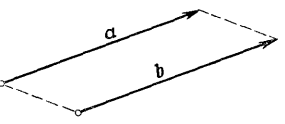
\includegraphics[width=0.3\textwidth]{image1_2.png}
    \end{figure}
  \item \textbf{Скользящие и приложенные векторные величины.} \\
  Если векторная величина определяется численной мерой, направлением и точкой приложения, то она называется \textit{приложенной}. \\
      \begin{figure}[H]
        \centering
        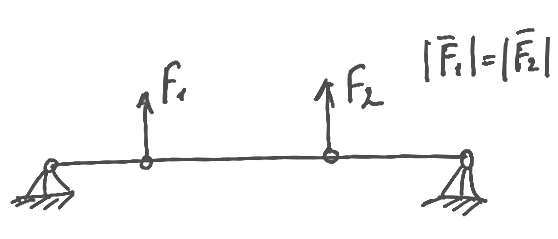
\includegraphics[width=0.3\textwidth]{image1_3.png}
    \end{figure}
  Если векторная величина определеяется численной мерой, направлением и прямой линией, имеющей это направление, то она называется \textit{скользящей}. \\
      \begin{figure}[H]
        \centering
        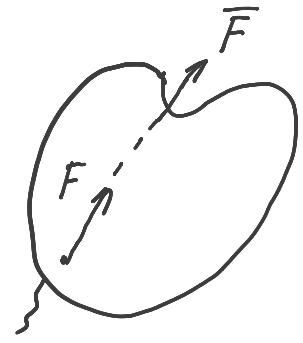
\includegraphics[width=0.2\textwidth]{image1_4.png}
    \end{figure}
  Если векторная величина определяется численной мерой и направлением, то она называется \textit{свободной}. У такой величины нет физического смысла.\\
  \item \textbf{Модуль вектора.} \textit{Модуль вектора} - скалярная величина, равная его длине при условии, что выбрана определённая единица измерения. $$|\vec{a}| = a$$
  \textit{Нулевой вектор} - вектор называется нулевым тогда и только тогда, когда его модуль равен нулю.
  \item \textbf{Орт вектора.} \textit{Ортом} данного вектора называется вектор, который направлен одинаково с данным вектором и имеет модуль, равный единице.
  $$\vec{a}_{0} = \frac{\vec{a}}{|\vec{a}|}$$
  \textit{Следствие}: равные векторы имеют равные орты.
  \item \textbf{Угол между векторами.} \textit{Угол между векторами} - меньшая часть плоскости, ограниченная двумя лучами, исходящими из одной точки и направленными одинаково с данными векторами. $0 < \phi < \pi$
    \begin{figure}[H]
        \centering
        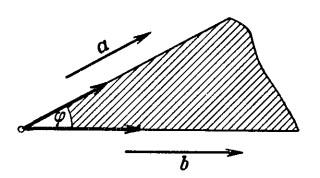
\includegraphics[width=0.3\textwidth]{image1_1.png}
    \end{figure}
\end{itemize}


\subsection{Операции над векторами:}
\begin{enumerate}
  \item \textbf{Сумма двух векторов.} \textit{Суммой} двух векторов $\vec{a}$ и $\vec{b}$ является третий вектор $\vec{R}$, соединяющий начало первого слагаемого вектора $\vec{a}$ с концом второго слагаемого при условии, что начало второго слагаемого совмещено с концом первого. Результат сложения не зависит от того, в какой точке пространства помещено начало первого слагаемого.
  \begin{figure} [H]
      \centering
      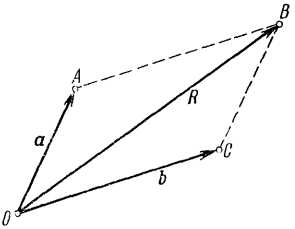
\includegraphics[width=0.3\linewidth]{image1_6.png}
  \end{figure}
  Операция нахождения суммы векторов называется \textit{сложением}. Для обозначения употребляется плюс:
  $$\vec{R} = \vec{a} + vec{b}$$
  \item \textbf{Сумма более чем двух векторов.} Сложение многих векторов $\vec{a}$, $\vec{b}$, $\vec{c}$, $\vec{d}$ ... совершается последовательно: сначала $\vec{a}$ и $\vec{b}$, затем к сумме $\vec{a} + \vec{b}$ прибавляется $\vec{c}$ и тд.
  \begin{figure} [H]
      \centering
      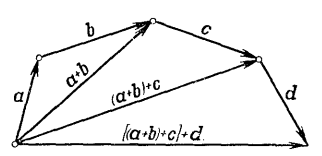
\includegraphics[width=0.3\linewidth]{image1_5.png}
  \end{figure}
  \textit{Правило многоугольника}: суммой нескольких векторов является вектор, соединяющий начало первого слагаемого вектора с концом последнего при условии, что начало каждого последующего вектора совмещено с концом предыдщего.\\ 
  \textbf{Законы сложения:}
    \begin{enumerate}
        \item \textit{Закон сочетательности.} Сумма не изменится, если любую группу последовательных слагаемых заменить их суммой:
        $$(\vec{a}+\vec{b})+\vec{c} = \vec{a} + (\vec{b}+\vec{c})$$
        \item \textit{Закон переместительности.} От перестановки мест слагаемых сумма не меняется:
        $$\vec{a}+\vec{b} = \vec{b}+\vec{a}$$
    \end{enumerate}
  \item \textbf{Модуль суммы.} Модуль суммы векторов не превосходит суммы модулей слагаемых:
  $$|\vec{a}+\vec{b}| \leqslant |\vec{a}| + |\vec{b}|$$
  \textit{Замечание}: Если слагаемые векторы имеют одинаковые направления, то модуль суммы равен сумме модулей: 
  $$|\vec{a}+\vec{b}| = |\vec{a}| + |\vec{b}|$$
  Если два слагаемых вектора имеют противоположные направления, то модуль их суммы равен разности модулей, причём из большего модуля вычитается меньший:
  $$|\vec{a}+\vec{b}| = |\vec{a}| - |\vec{b}|$$
  \item \textbf{Вычитание векторов.} Разностью двух векторов $\vec{a}$ и $\vec{b}$, из которых первый именуется \textit{уменьшаемым}, а второй - \textit{вычитаемым}, называется сумма уменьшаемого вектора и вектора, противоположного вычитаемому.
  $$\vec{a}-\vec{b} = \vec{a}+(-\vec{b})$$
  \begin{figure}[H]
      \centering
      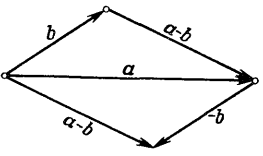
\includegraphics[width=0.26\linewidth]{image1_7.png}
  \end{figure}
  \textit{Противоположный вектор} - вектор, имеющий модуль, равный исходному, но противоположное направление.\\
  Сумма двух противоположных векторов равна нулю:
  $$\vec{a}+(-\vec{a}) = 0$$
  Вектор, противоположный противоположному, совпадает с исходным:
  $$-(-\vec{a}) = \vec{a}$$
  \item \textbf{Вычитание как операция, обратная сложению.} Из вычитания векторов видно, что $ \vec{b} + (\vec{a} - \vec{b}) = \vec{a}$, т.е. сумма разности и вычитаемого вектора равна уменьшаемому вектору. \\
  Операция вычитания векторов есть операция, обратная сложению: при её помощи по сумме $\vec{a}$ и одному слагаемому $\vec{b}$ находится второе слагаемое $\vec{a} - \vec{b}$.
  \item \textbf{Умножение вектора на скаляр.} Умножение вектора на целое положительное число $n$ можно считать как сложение вектора $n$ раз. \\
  Произведением вектора и скаляра называется новый вектор, который имеет:
  \begin{enumerate}
      \item модуль, равный произведению модуля умножаемого вектора на абсолютную величину скаляря;
      \item направление, одинаковое с умножаемым вектором, если скаляр положительный, и противоположно, если скаляр отрицательный.
  \end{enumerate}
  Произведение вектора $\vec{a}$ и скаляра $\lambda$ обозначается $\vec{a}\lambda$ или $\lambda\vec{a}$, таким образом:
  $$|\lambda\vec{a}| = |\vec{a}\lambda| = |\lambda|*|\vec{a}|$$
  \textit{Замечание}: из определения следует, что произведение равно нулю тогда и только тогда, когда один из множителей равен нулю:
  $$\lambda*\vec{0} = \vec{0}; 0*\vec{a} = \vec{0}$$
  \textbf{Законы умножения вектора на скаляр}:
  \begin{enumerate}
      \item \textit{Закон сочетательности для скалярных множителей}. Последовательное умножение вектора на несколько скалярных множителей равносильно умножению вектора на произведение этих множителей:
      $$\lambda(\mu \vec{a}) = (\lambda \mu) \vec{a}$$
      \item \textit{Закон двоякой распределительности}. Умножение суммы векторов на скаляр, а также умножение суммы скаляров на вектор можно производить почленно:
      $$(\vec{a}+\vec{b})\lambda = \vec{a}\lambda+\vec{b}\lambda$$
      $$(\lambda+\mu)\vec{a} = \lambda\vec{a} + \mu \vec{a}$$
  \end{enumerate}
  \item \textbf{Деление вектора на скаляр.} Деление вектора на скаляр определяется как умножение этого вектора на обратный скаляр:
  $$\frac{\vec{a}}{\lambda} = \frac{1}{\lambda}\vec{a}$$
  \item \textbf{Выражение вектора серез его модуль и орт.} Если умножить орт вектора на модуль вектора, то получится сам вектор:
  $$\vec{a} = a*\vec{a}_{0}$$
  \item  \textbf{Линейная комбинация.} Если над векторами $\vec{a}$, $\vec{b}$, $\vec{c}$, $\vec{d}$ выполнять действия сложения, вычитания, умножения на скаляр, то в результате любого числа таких действий получается вектор вида
  $$\alpha \vec{a} + \beta \vec{b} + \gamma \vec{c} + \delta \vec{d}$$
  представляющий собой \textit{линейную комбинацию} исходных векторов.
\end{enumerate}


\subsection{Линейные зависимости между векторами:}
\begin{enumerate}
    \item \textbf{Линейно зависимые вектора.} Вектора $\vec{a}$, $\vec{b}$, $\vec{c}$, $\vec{d}$ являются линейно зависимыми, если между ними выполняется соотношение вида:
     $$\alpha \vec{a} + \beta \vec{b} + \gamma \vec{c} + \delta \vec{d} = 0$$
     \item \textbf{Коллениарные вектора.} Вектора называются коллениарными, если они параллельны одной прямоы. Нулевой вектор считается коллениарным любому вектору. \\
     \textit{Теорема.} Два вектора линейно зависимы тогда и только тогда, когда они коллинеарны. \\
     \textit{Следствие.} Если между двумя неколлениарными векторами выполняется линейное соотношение
     $$\alpha\vec{a} + \beta\vec{b} = 0$$
     то оба скалярных коэффициента должны равняться нулю.
     \item \textbf{Компланарыне векторы.} Векторы называются компланарными, если они параллельны одной плоскости. Нулевой вектор считается компланарным любой системе компланарынх векторов.\\
     \textit{Теорема.} Три вектора линейно зависимы тогда и только тогда, когда они компланарны. \\
     \textit{Следствие.} Если между тремя некомпланарными векторами выполняется линейное соотношение
     $$\alpha\vec{a} + \beta\vec{b} + \gamma\vec{c} = 0$$
     то все три скалярных коэффициента должны равняться нулю.
\end{enumerate}


\subsection{Произведения двух векторов:}
\begin{enumerate}
    \item \textbf{Скалярное произведение двух векторов.} Скалярное произвеление двух векторов называется произвеление их модулей на косинус угла между ними.
    $$\vec{a}*\vec{b} = |\vec{a}|*|\vec{b}|*\cos\phi$$
    \textit{Равенство скалярного произведения нулю.} Скалярное произведение двух векторов равно нулю тогда и только тогла, когда хотя бы один из перемножаемых векторов равен нулю или когда эти вектора перпендикулярны, т.е. условием перпендикулярности ненулевых векторов является равенство нулю их скалярного произведение. \\
    Законы скалярного умножения:
    \begin{enumerate}
        \item \textit{Закон переместительности.} Скалярное произведение не меняется от перестановки множителей
        $$\vec{a}*\vec{b} = \vec{b} * \vec{a}$$
        \item \textit{Закон распределительности.} Скалярное умножение вектора на сумму векторов можно производить почленно, т.е.
        $$\vec{a}*(\vec{b}+\vec{c}) = \vec{a}*\vec{b}+\vec{a}*\vec{c}$$
        \textit{Лемма.} Скалярное произведение равно произведения модуля одного вектора на проекцию другого на первый:
        $$\vec{p}*\vec{q} = p*np_{\vec{p}}\vec{q}$$
        \item \textit{Закон сочетательности относительно скалярных множителей.} Скалярное произвеление не изменится, если скалярный множитель вынести за скобки:
        $$(\lambda\vec{a})*\vec{b} = \lambda(\vec{a}*\vec{b})$$
    \end{enumerate}
    \item \textbf{Векторное произведение двух векторов.} Векторным произведение двух векторов $\vec{a}$ и $\vec{b}$ называется третий вектор $\vec{N}$, который:
    \begin{enumerate}
        \item имеет модуль, численно ранвый площади параллелограмма, построенного на перемножаемых векторах;
        \item направлен перпендикулярно к перемножаемым векторам в ту сторону, откуда наименьший поворот первого множителя, совмещающий его направление с направлением второго множителя, виде проиходящим против хода часовой стрелки(правило правой руки).
    \end{enumerate}
    $$\vec{a}\times\vec{b}$$
    $$\vec{N} = \vec{a}\times\vec{b}$$
    Модуль векторого произведения:
    $$|\vec{a}\times\vec{b}| = |\vec{a}|*|\vec{b}|*\sin\phi$$
    \textit{Условия равенства нулю векторого произведения.} Векторное произведение двух векторов равно нулю тогда и только тогда, когда хотя бы один из перемножаемых векторов равен нулю или когда эти вектора коллинеарны. \\
    Законы векторного умножения:
    \begin{enumerate}
        \item \textit{Закон противопереместительности.} При перестановке множителей векторное произведение меняет только свой знак
        $$\vec{a}\times\vec{b} = -(\vec{b}\times\vec{a})$$
        \item \textit{Закон распределительности.} Векторное умножение вектора на сумму векторов можно производить почленно
        $$(\vec{a}+\vec{b})\times\vec{c} = \vec{a}\times\vec{c} + \vec{b}\times\vec{c} $$
        \item \textit{Закон сочетательности относительно скалярных множителей.} Скалярный множитель можно вынести за зак векторного произведения
        $$(\lambda\vec{a})\times\vec{b} = \lambda(\vec{a}\times\vec{b})$$
    \end{enumerate}
\end{enumerate}


\section{Семинар 2}

  \subsection{Производная вектора постоянного модуля}
  Первый замечательный предел:
  $$\lim_{x \rightarrow 0} \frac{\sin x}{x} = 1$$
  Производная функции в общем виде:
  $$f'(x) = \lim_{\Delta x \rightarrow 0} \frac{f(x + \Delta x) - f(x)}{\Delta x}$$

  \subsubsection{Вектор-функция скалярного аргумента}
  \par Рассмотрим вектор-функцию, зависящую от скаляра $\vec{r} = \vec{r}(t)$.\\
  В координатном виде данная функция может быть задана как 
  $$r_x = r_x(t), r_y=r_y(t), r_z = r_z(t)$$ 
  Таким образом и сам вектор может быть задан через главные орты: 
  $$\vec{r}(t) = r_x(t)\cdot\vec{i}+r_y(t)\cdot\vec{j}+r_z(t)\cdot\vec{k}$$

  \textbf{Годограф вектора.} Годографом вектора, зависящего от скаляра, называется кривая, которую описывает конец вектора-функции, когда его начало помещено в 0.
  \begin{figure}[H]
      \centering
    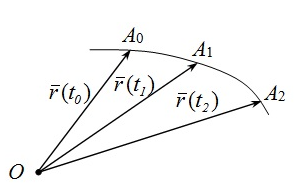
\includegraphics[width=0.25\textwidth]{image2_4.png}
  \end{figure}

  \subsubsection{Производная вектора по скалярному аргументу}

  \par\textbf{Производная вектора.} Производной вектора по его скалярному аргументу называется предел отношения приращения вектора к соответствующему приращению скалярного аргумента, когда приращение этого аргумента стремится к нулю.\\
  \begin{figure}[H]
      \centering
    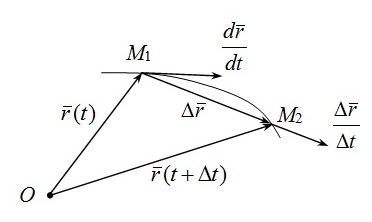
\includegraphics[width=0.3\textwidth]{image2_5.png}
  \end{figure}
  Найдём отношение приращения вектора к приращению аргумента.
  $$\frac {\Delta \vec{r}} {\Delta t} = \frac{\vec{r}(t+\Delta t) - \vec{r}(t)}{\Delta t}$$
  При стремлении $\Delta t \rightarrow 0$:
  $$\frac{d\vec{r}}{dt} = \lim_{\Delta t \rightarrow 0} \frac{\Delta \vec{r}}{\Delta t}$$
  $$\dot{\vec{r}} = \frac{d\vec{r}}{dt}$$
  \par\textbf{Геометрический смысл производной вектора.} Производная вектора по его скалярному аргументу есть вектор, направленной по касательной к годографу исходного вектора в рассматриваемой точке.\\
  \textit{Замечание.} Производная направлена по касательной в ту сторону, куда перемещается конец вектора, когда параметр растёт.
  \par\textbf{Механический смысл производной вектора.} Производная радиус-вектора движущейся точки по времени есть скорость этой точки в данный момент.
  $$\omega = \lim_{\Delta t \rightarrow 0} \frac{\Delta r}{\Delta t} = \dot{r}$$
  \textit{Замечание.} Производную вектора можно всегда рассматривать как скорость конца вектора при условии, что его начало всегда находится в фиксированной точке, а аргумент рассматривается как время.
  \begin{figure}[H]
      \centering
    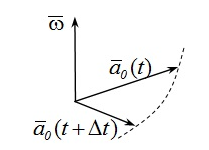
\includegraphics[width=0.2\textwidth]{image2_2.png}
  \end{figure}
  \subsubsection{Правила дифференцирования вектора по скаляру.}
  \begin{enumerate}
    \item определение производной вектора по скаляру совпадает с обычным определением;
    \item теоремы о пределах векторных вращений не отличаются от обычных теорем о пределах;
    \item векторные алгебраические операции подчиняются законам алгебры.
  \end{enumerate}

  \subsubsection{Свойства производной от вектора по скалярному аргументу}
  \begin{enumerate}
    \item Если вектор $\vec{a}$ постоянен, т.е. не меняет со временем ни модуля, ни направления, то $\frac{d\vec{a}}{dt} = 0$;
    \item $\frac {d}{dt} (\vec{a}+\vec{b}) = \frac{d\vec{a}}{dt} +\frac{d\vec{b}}{dt}$, $\frac {d}{dt} (\vec{a}\cdot\vec{b}) = \frac{d\vec{a}}{dt}\cdot\vec{b} + \frac{d\vec{b}}{dt}\cdot\vec{a}$
    \item Если аргументом вектора $\vec{a}$ является сложна функция $S = S(t)$, т.е.
    $\vec{a} = \vec{a}(S(t))$, $\frac{d\vec{a}}{dt} = \frac{d\vec{a}}{dS}\cdot\frac{dS}{dt}$
  \end{enumerate}

  \subsubsection{Производная вектора постоянного модуля}
  Будем рассматривать вектор $\vec{a}(t)$, который является переменным, но постоянным по модулю. Т.е.:
  \begin{enumerate}
    \item $|\vec{a}(t)| = const \neq 0$
    \item $\vec{a}(t+\Delta t)$ и $\vec{a}(t)$ неколлинеарны хотя бы в некоторых точка t в пределах его одз.
  \end{enumerate}
  \begin{figure}[H]
      \centering
    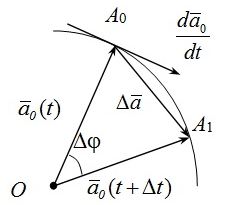
\includegraphics[width=0.2\textwidth]{image2_6.png}
  \end{figure}

  \subsubsection{Направление производной вектора постоянного модуля} 
  (Годограф вектора с постоянным модулем выглядит как окружность.)\\
  \par\textit{Доказательство1.} Запишем скалярное произведение двух векторов $\vec{a}\cdot\vec{a} = a^2 = const$, возьмём производную от левой части:
  $$\frac{d}{dt}(\vec{a}\cdot\vec{a}) = \frac{d}{dt}(a^2)$$
  Распишем подробнее производную:
  $$\dot{\vec{a}}\cdot\vec{a} + \vec{a}\cdot\dot(\vec{a}) = 0$$
  $$2\dot{\vec{a}}\cdot\vec{a} = 0$$
  Из чего следует, что вектора $\vec{a}$ и $\dot{\vec{a}}$ перпендикулярны, т.е. $\cos(\vec{a};\dot{\vec{a}}) = \pm\frac{\pi}{2}$\\
  \par\textit{Доказательство2.} У нас есть годограф вектора $\vec{a}$. Если модуль вектора равен константе $|\vec{a}| = const$, то модуль годографа вектора постоянен => Годограф это окружность или часть окружности. И таким образом касательная $\dot{\vec{r}}(t)$ перпендикулярна радиусу $\vec{r}(t)$ по свойству окружности.
  \par Модуль вектора $\vec{a}(t)$.\\
  $$\Delta \vec{a} = \vec{a}(t+\Delta t) - \vec{a}(t)$$
  $$|\Delta \vec{a}| = \Delta a = 2a\sin\phi$$
  $$\frac{\Delta a}{\Delta t} = \frac{2a\sin\Delta\phi}{\Delta t}$$
  По определению модуль производной:
  $$|\dot{\vec{a}}| = \lim_{\Delta t \rightarrow 0}\frac{\Delta a}{\Delta t} = a \cdot \lim_{\Delta t \rightarrow 0}\frac{2\sin\Delta\phi}{\Delta t} = a \cdot \lim_{\Delta t \rightarrow 0}\frac{2\sin\Delta\phi}{\Delta \phi}\cdot\frac{\Delta\phi}{\Delta t} = a\cdot\lim_{\Delta \phi \rightarrow 0}\frac{\sin\Delta\phi}{\Delta\phi}\cdot\lim_{\Delta \rightarrow 0} \frac{2\Delta\phi}{\Delta t} = a \cdot\lim_{\Delta t \rightarrow}\frac{\Delta\psi}{\Delta t} = a\cdot\dot{\psi}$$

  $\dot{\vec{a}}: |\dot{\vec{a}}| = a\cdot\dot{\psi}$, где $\dot{\psi}$ - скорость поворота вектора.\\
  Так как $\dot{\psi} = \omega$ перпендикулярна плоскости годографа, то можно сказать, что
  $$\dot{\vec{a}} = \vec{a}\times\vec{\omega}$$

  Введём вектор $\vec{k} = \vec{a}_{o} \times \dot{\vec{a}}_{o}$, $\vec{\omega} = \dot{\psi}\vec{k}$, где $k$ - скорость поворота орт-вектора.



  \subsection{Понятия кривизны и радиуса кривизны}

  \par Пускай есть некоторый радиус $\vec{r}$, тогда кривизной радиуса в точке называют величину $K$.
  $$K = \lim_{\Delta S \rightarrow 0}\frac{\Delta \phi}{\Delta S} = \frac{d\phi}{dS}$$
  \begin{figure}[H]
      \centering
    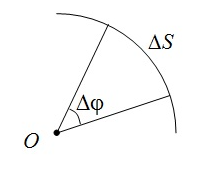
\includegraphics[width=0.2\textwidth]{image2_1.png}
  \end{figure}
  \textit{Радиус кривизны} $\rho$ -- обратная величина к кривизне.
  $$\rho = \frac{1}{K} = \frac{dS}{d\phi}$$

  \subsection{Примеры}
  \subsubsection*{Пример1}
  Пускай есть вектор $\vec{b}(t) = 1\cdot\vec{i}+2\cdot\vec{j}+3\cdot\vec{k}$ в декартовой системе координат. Как у этого вектора найти $\dot{\vec{b}}(t)$?
  Является ли этот вектор переменным, т.е. зависит ли он от \textit{t}?\\ 
  \textit{Решение:} Нет, соответственно $\dot{\vec{b}}(t) = 0$, а модуль $|\vec{b}| = 14$.\\
  \subsubsection*{Пример2}
  $\vec{b}(t) = \cos(\omega_{0}t)\vec{i}+\sin(\omega_{0}t)\vec{j}$. $t = 0$, $\vec{\omega}$, $\dot{\vec{b}}$ -- ?\\
  \textit{Решение:} $\dot{\vec{b}}(t) = -\omega_{0}\cdot\sin(\omega_{0}t)\vec{i}+\omega_{0}\cdot\cos(\omega_{0}t)\vec{j}$; $|\vec{b}| = \omega_{0}$\\
  $\frac{d\vec{i}}{dt} = 0$, $\frac{d\vec{j}}{dt} = 0$\\
  \begin{figure}[H]
      \centering
    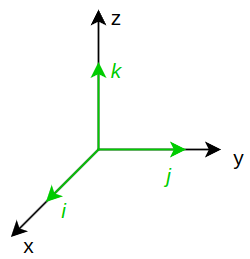
\includegraphics[width=0.2\textwidth]{image2_3.png}
  \end{figure}
  \subsubsection*{Пример3}
  $|\vec{b}|=\sin(\omega_{0}t)\vec{i}+\cos(\omega_{0}t)\vec{j}$, $|\vec{b}| = 1$, $\dot{\vec{b}}$, $\vec{\omega}$ -- ? при t = 0\\
  \textit{Решение:}
  $$t = \frac{\pi}{4\omega_{0}}\cdot k, k \in Z$$
  $$\dot{\vec{b}} = \omega_{0}\cdot\cos(\omega_{0}t)\vec{i} - \omega_{0}\cdot\sin(\omega_{0}t)\vec{j}$$
  $$|\dot{\vec{b}}| = |\vec{\omega}|\cdot|\vec{b}|\cdot\sin\phi, \vec{\omega}\bot\vec{b}$$
  $$|\dot{\vec{b}}| = |\vec{\omega}|\cdot|\vec{b}|$$ откуда 
  $$|\vec{\omega}| = \sqrt{\omega_{0}^{2}\cdot \cos^2(\omega t)+\omega_{0}^{2}\cdot \sin^2(\omega t)} = \omega_{0}\sqrt{\cos^2(\omega_0 t)+\sin^2(\omega_0 t)} = \omega_{0}$$
  $$|\vec{b}|=\sqrt{\omega_{0}^2\cdot\sin^2(\omega_{0}t)+\omega_{0}^2\cdot\cos^2(\omega_{0}t)} = \omega_{0}\sqrt{\sin^2(\omega_0 t)+\cos^2(\omega_0 t)} = \omega_{0}$$
  $$|\dot{\vec{b}}| = \omega_{0}^2$$
  $$|\vec{\omega}| = \frac{|\dot{\vec{b}}|}{|\vec{b}|} = \omega_{0}$$
  
  \subsubsection*{Пример 4}
  $$\vec{b}(t) = \frac{t}{\sqrt{t^2+1}}\cdot\vec{i}+\frac{1}{\sqrt{t^2+1}}\cdot\vec{j}$$ при $t = 0$.\\
  $|\dot{\vec{b}}|, |\vec{\omega}|$ -- ? \\
  \textit{Решение:}
  $$\dot{\vec{b}}(t) = \frac{1}{\sqrt{t^2+1}(t^2+1)}\cdot\vec{i}-\frac{t}{\sqrt{t^2+1}(t^2+1)}\cdot\vec{j}$$
  $$|\dot{\vec{b}}| = |\vec{\omega}|\cdot|\vec{b}|\cdot\sin\phi, \vec{\omega}\bot\vec{b}$$
  откуда
  $$|\vec{b}| = \sqrt{b_{i}^2+b_{j}^2} = \sqrt{\frac{1}{(t^2+1)^3}+\frac{t^2}{(t^2+1)^3}}=\sqrt{\frac{t^2+1}{(t^2+1)^3}}=\frac{1}{|t^2+1|}$$




\end{document}

